\documentclass{article}\usepackage[]{graphicx}\usepackage[]{xcolor}
% maxwidth is the original width if it is less than linewidth
% otherwise use linewidth (to make sure the graphics do not exceed the margin)
\makeatletter
\def\maxwidth{ %
  \ifdim\Gin@nat@width>\linewidth
    \linewidth
  \else
    \Gin@nat@width
  \fi
}
\makeatother

\definecolor{fgcolor}{rgb}{0.345, 0.345, 0.345}
\newcommand{\hlnum}[1]{\textcolor[rgb]{0.686,0.059,0.569}{#1}}%
\newcommand{\hlstr}[1]{\textcolor[rgb]{0.192,0.494,0.8}{#1}}%
\newcommand{\hlcom}[1]{\textcolor[rgb]{0.678,0.584,0.686}{\textit{#1}}}%
\newcommand{\hlopt}[1]{\textcolor[rgb]{0,0,0}{#1}}%
\newcommand{\hlstd}[1]{\textcolor[rgb]{0.345,0.345,0.345}{#1}}%
\newcommand{\hlkwa}[1]{\textcolor[rgb]{0.161,0.373,0.58}{\textbf{#1}}}%
\newcommand{\hlkwb}[1]{\textcolor[rgb]{0.69,0.353,0.396}{#1}}%
\newcommand{\hlkwc}[1]{\textcolor[rgb]{0.333,0.667,0.333}{#1}}%
\newcommand{\hlkwd}[1]{\textcolor[rgb]{0.737,0.353,0.396}{\textbf{#1}}}%
\let\hlipl\hlkwb

\usepackage{framed}
\makeatletter
\newenvironment{kframe}{%
 \def\at@end@of@kframe{}%
 \ifinner\ifhmode%
  \def\at@end@of@kframe{\end{minipage}}%
  \begin{minipage}{\columnwidth}%
 \fi\fi%
 \def\FrameCommand##1{\hskip\@totalleftmargin \hskip-\fboxsep
 \colorbox{shadecolor}{##1}\hskip-\fboxsep
     % There is no \\@totalrightmargin, so:
     \hskip-\linewidth \hskip-\@totalleftmargin \hskip\columnwidth}%
 \MakeFramed {\advance\hsize-\width
   \@totalleftmargin\z@ \linewidth\hsize
   \@setminipage}}%
 {\par\unskip\endMakeFramed%
 \at@end@of@kframe}
\makeatother

\definecolor{shadecolor}{rgb}{.97, .97, .97}
\definecolor{messagecolor}{rgb}{0, 0, 0}
\definecolor{warningcolor}{rgb}{1, 0, 1}
\definecolor{errorcolor}{rgb}{1, 0, 0}
\newenvironment{knitrout}{}{} % an empty environment to be redefined in TeX

\usepackage{alltt}
\usepackage[sc]{mathpazo}
\renewcommand{\sfdefault}{lmss}
\renewcommand{\ttdefault}{lmtt}
\usepackage[T1]{fontenc}
\usepackage{geometry}
\geometry{verbose,tmargin=2.5cm,bmargin=2.5cm,lmargin=2.5cm,rmargin=2.5cm}
\setcounter{secnumdepth}{2}
\setcounter{tocdepth}{2}
\usepackage[unicode=true,pdfusetitle,
 bookmarks=true,bookmarksnumbered=true,bookmarksopen=true,bookmarksopenlevel=2,
 breaklinks=false,pdfborder={0 0 1},backref=false,colorlinks=false]
 {hyperref}
\hypersetup{
 pdfstartview={XYZ null null 1}}

\makeatletter
%%%%%%%%%%%%%%%%%%%%%%%%%%%%%% User specified LaTeX commands.
\renewcommand{\textfraction}{0.05}
\renewcommand{\topfraction}{0.8}
\renewcommand{\bottomfraction}{0.8}
\renewcommand{\floatpagefraction}{0.75}

\makeatother
\IfFileExists{upquote.sty}{\usepackage{upquote}}{}
\begin{document}








The results below are generated from an R script.

\begin{knitrout}
\definecolor{shadecolor}{rgb}{0.969, 0.969, 0.969}\color{fgcolor}\begin{kframe}
\begin{alltt}
\hlcom{# Question 1}
\hlcom{#a.}
\hlstd{chickwts[}\hlnum{14}\hlstd{,]}
\end{alltt}
\begin{verbatim}
##    weight    feed
## 14    141 linseed
\end{verbatim}
\begin{alltt}
\hlcom{#b.}
\hlstd{chickwts}\hlopt{$}\hlstd{weight[}\hlkwd{c}\hlstd{(}\hlnum{7}\hlstd{,}\hlnum{14}\hlstd{,}\hlnum{37}\hlstd{)]}
\end{alltt}
\begin{verbatim}
## [1] 108 141 423
\end{verbatim}
\begin{alltt}
\hlcom{#c.}
\hlstd{chickwtsCasein} \hlkwb{<-} \hlstd{chickwts[chickwts}\hlopt{$}\hlstd{feed} \hlopt{==} \hlstr{"casein"}\hlstd{, ]}
\hlstd{chickwtsCasein}
\end{alltt}
\begin{verbatim}
##    weight   feed
## 60    368 casein
## 61    390 casein
## 62    379 casein
## 63    260 casein
## 64    404 casein
## 65    318 casein
## 66    352 casein
## 67    359 casein
## 68    216 casein
## 69    222 casein
## 70    283 casein
## 71    332 casein
\end{verbatim}
\begin{alltt}
\hlcom{#d. }
\hlkwd{mean}\hlstd{(chickwtsCasein}\hlopt{$}\hlstd{weight)}
\end{alltt}
\begin{verbatim}
## [1] 323.5833
\end{verbatim}
\begin{alltt}
\hlcom{#e.}
\hlstd{Feed} \hlkwb{=} \hlkwd{levels}\hlstd{(chickwts}\hlopt{$}\hlstd{feed)}
\hlstd{Feed}
\end{alltt}
\begin{verbatim}
## [1] "casein"    "horsebean" "linseed"   "meatmeal"  "soybean"   "sunflower"
\end{verbatim}
\begin{alltt}
\hlcom{#f.}
\hlstd{chick240} \hlkwb{=} \hlkwd{subset}\hlstd{(chickwts, chickwts}\hlopt{$}\hlstd{weight}\hlopt{<}\hlnum{240}\hlstd{)}
\hlstd{chick240}
\end{alltt}
\begin{verbatim}
##    weight      feed
## 1     179 horsebean
## 2     160 horsebean
## 3     136 horsebean
## 4     227 horsebean
## 5     217 horsebean
## 6     168 horsebean
## 7     108 horsebean
## 8     124 horsebean
## 9     143 horsebean
## 10    140 horsebean
## 12    229   linseed
## 13    181   linseed
## 14    141   linseed
## 16    203   linseed
## 17    148   linseed
## 18    169   linseed
## 19    213   linseed
## 24    230   soybean
## 29    193   soybean
## 33    199   soybean
## 34    171   soybean
## 35    158   soybean
## 42    226 sunflower
## 54    153  meatmeal
## 57    206  meatmeal
## 68    216    casein
## 69    222    casein
\end{verbatim}
\begin{alltt}
\hlcom{#g.}
\hlstd{chick240Table} \hlkwb{=} \hlkwd{table}\hlstd{(chick240}\hlopt{$}\hlstd{feed)}
\hlstd{chick240Table}
\end{alltt}
\begin{verbatim}
## 
##    casein horsebean   linseed  meatmeal   soybean sunflower 
##         2        10         7         2         5         1
\end{verbatim}
\begin{alltt}
\hlkwd{barplot}\hlstd{(chick240Table)}
\end{alltt}
\end{kframe}

{\centering 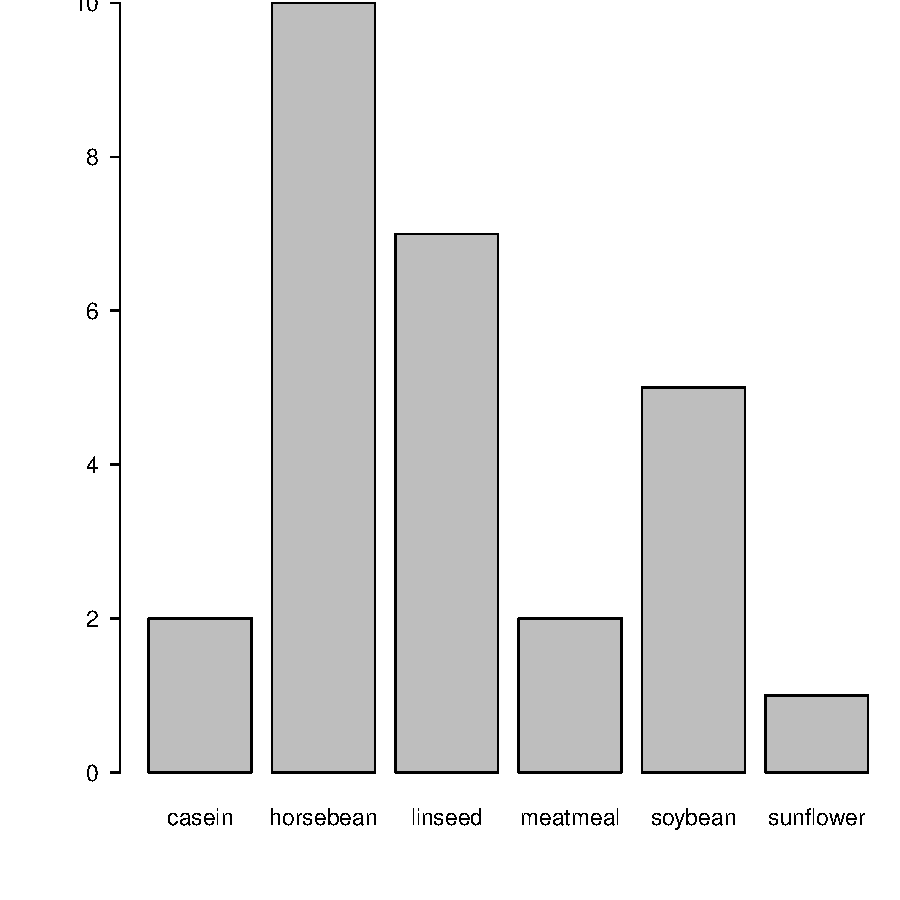
\includegraphics[width=.6\linewidth]{figure/Meng51940633A2-Rnwauto-report-1} 

}


\begin{kframe}\begin{alltt}
\hlcom{#Question 2}
\hlcom{#a.}
\hlkwd{nrow}\hlstd{(cuckoos)}
\end{alltt}


{\ttfamily\noindent\bfseries\color{errorcolor}{\#\# Error in nrow(cuckoos): object 'cuckoos' not found}}\begin{alltt}
\hlcom{#b.}
\hlstd{cuckoos}\hlopt{$}\hlstd{length[}\hlnum{27}\hlstd{]}
\end{alltt}


{\ttfamily\noindent\bfseries\color{errorcolor}{\#\# Error in eval(expr, envir, enclos): object 'cuckoos' not found}}\begin{alltt}
\hlcom{#c.}
\hlstd{cuckoos[}\hlnum{40}\hlstd{,]}
\end{alltt}


{\ttfamily\noindent\bfseries\color{errorcolor}{\#\# Error in eval(expr, envir, enclos): object 'cuckoos' not found}}\begin{alltt}
\hlcom{#d.}
\hlstd{cuckoosSpecies} \hlkwb{=} \hlkwd{levels}\hlstd{(cuckoos}\hlopt{$}\hlstd{species)}
\end{alltt}


{\ttfamily\noindent\bfseries\color{errorcolor}{\#\# Error in levels(cuckoos\$species): object 'cuckoos' not found}}\begin{alltt}
\hlstd{cuckoosSpecies}
\end{alltt}


{\ttfamily\noindent\bfseries\color{errorcolor}{\#\# Error in eval(expr, envir, enclos): object 'cuckoosSpecies' not found}}\begin{alltt}
\hlcom{#e.}
\hlstd{cuckoos}\hlopt{$}\hlstd{m.pipitFactor} \hlkwb{=} \hlstd{cuckoos}\hlopt{$}\hlstd{species}
\end{alltt}


{\ttfamily\noindent\bfseries\color{errorcolor}{\#\# Error in eval(expr, envir, enclos): object 'cuckoos' not found}}\begin{alltt}
\hlkwd{levels}\hlstd{(cuckoos}\hlopt{$}\hlstd{m.pipitFactor)} \hlkwb{=} \hlkwd{c}\hlstd{(}\hlstr{"other"}\hlstd{,}\hlstr{"meadow.pipit"}\hlstd{,} \hlkwd{rep}\hlstd{(}\hlstr{"other"}\hlstd{,}\hlnum{4}\hlstd{))}
\end{alltt}


{\ttfamily\noindent\bfseries\color{errorcolor}{\#\# Error in levels(cuckoos\$m.pipitFactor) = c("{}other"{}, "{}meadow.pipit"{}, rep("{}other"{}, : object 'cuckoos' not found}}\begin{alltt}
\hlkwd{levels}\hlstd{(cuckoos}\hlopt{$}\hlstd{m.pipitFactor)}
\end{alltt}


{\ttfamily\noindent\bfseries\color{errorcolor}{\#\# Error in levels(cuckoos\$m.pipitFactor): object 'cuckoos' not found}}\begin{alltt}
\hlstd{cuckoos}\hlopt{$}\hlstd{m.pipitFactor}\hlopt{==}\hlstr{"meadow.pipit"}
\end{alltt}


{\ttfamily\noindent\bfseries\color{errorcolor}{\#\# Error in eval(expr, envir, enclos): object 'cuckoos' not found}}\begin{alltt}
\hlcom{#g.}
\hlstd{cuckoosMPipit} \hlkwb{=} \hlkwd{subset}\hlstd{(cuckoos, m.pipitFactor}\hlopt{==}\hlstr{"meadow.pipit"}\hlstd{)}
\end{alltt}


{\ttfamily\noindent\bfseries\color{errorcolor}{\#\# Error in subset(cuckoos, m.pipitFactor == "{}meadow.pipit"{}): object 'cuckoos' not found}}\begin{alltt}
\hlstd{cuckoosMPipit}
\end{alltt}


{\ttfamily\noindent\bfseries\color{errorcolor}{\#\# Error in eval(expr, envir, enclos): object 'cuckoosMPipit' not found}}\begin{alltt}
\hlstd{cuckoosOther} \hlkwb{<-} \hlkwd{subset}\hlstd{(cuckoos, m.pipitFactor}\hlopt{==}\hlstr{"other"}\hlstd{)}
\end{alltt}


{\ttfamily\noindent\bfseries\color{errorcolor}{\#\# Error in subset(cuckoos, m.pipitFactor == "{}other"{}): object 'cuckoos' not found}}\begin{alltt}
\hlstd{cuckoosOther}
\end{alltt}


{\ttfamily\noindent\bfseries\color{errorcolor}{\#\# Error in eval(expr, envir, enclos): object 'cuckoosOther' not found}}\begin{alltt}
\hlcom{#h.}
\hlstd{cuckoosLongLength} \hlkwb{=} \hlkwd{subset}\hlstd{(cuckoos, length}\hlopt{>}\hlnum{23}\hlstd{)}
\end{alltt}


{\ttfamily\noindent\bfseries\color{errorcolor}{\#\# Error in subset(cuckoos, length > 23): object 'cuckoos' not found}}\begin{alltt}
\hlstd{cuckoosLongLength}
\end{alltt}


{\ttfamily\noindent\bfseries\color{errorcolor}{\#\# Error in eval(expr, envir, enclos): object 'cuckoosLongLength' not found}}\begin{alltt}
\hlkwd{mean}\hlstd{(cuckoosLongLength}\hlopt{$}\hlstd{breadth)}
\end{alltt}


{\ttfamily\noindent\bfseries\color{errorcolor}{\#\# Error in mean(cuckoosLongLength\$breadth): object 'cuckoosLongLength' not found}}\begin{alltt}
\hlcom{#Question 3}
\hlcom{#a.}
\hlstd{rain.df} \hlkwb{=} \hlkwd{read.table}\hlstd{(}\hlstr{"rain.txt"}\hlstd{,}\hlkwc{header}\hlstd{=}\hlnum{FALSE}\hlstd{,}\hlkwc{sep}\hlstd{=}\hlstr{""}\hlstd{)}
\hlstd{rain.df}
\end{alltt}
\begin{verbatim}
##    V1 V2 V3 V4 V5 V6 V7 V8 V9 V10 V11 V12 V13 V14 V15 V16 V17 V18 V19 V20 V21 V22 V23 V24
## 1  60  4  1  0  0  0  0  0  0   0   0   0   0   0   0   0   0   0   0   0   0   0   0   0
## 2  60  4  2  0  0  0  0  0  0   0   0   0   0   0   0   0   0   0   0   0   0   0   0   0
## 3  60  4  3  0  0  0  0  0  0   0   0   0   0   0   0   0   0   0   0   0   0   0   0   0
## 4  60  4  4  0  0  0  0  0  0   0   0   0   0   0   0   0   0   0   0   0   0   0   0   0
## 5  60  4  5  0  0  0  0  0  0   0   0   0   0   0   0   0   0   0   0   0   0   0   0   0
## 6  60  4  6  0  0  0  0  0  0   0   0   0   0   0   0   0   0   0   0   0   0   0   0   0
## 7  60  4  7  0  0  0  0  0  0   0   0   0   0   0   0   0   0   0   0   0   0   0   0   0
## 8  60  4  8  0  0  0  0  0  0   0   0   0   0   0   0   0   0   0   0   0   0   0   0   0
## 9  60  4  9  0  0  0  0  0  0   0   0   0   0   0   0   0   0   0   0   0   0   0   0   0
## 10 60  4 10  0  0  0  0  0  0   0   0   0   0   0   0   0   0   0   0   0   0   0   0   0
## 11 60  4 11  0  0  0  0  0  0   0   0   0   0   0   0   0   0   0   0   0   0   0   0   0
## 12 60  4 12  0  0  0  0  0  0   0   0   0   0   0   0   0   0   0   0   0   0   0   0   0
## 13 60  4 13  0  0  0  0  0  0   0   0   0   0   0   0   0   0   0   0   0   0   0   0   0
## 14 60  4 14  0  0  0  0  0  0   0   0   0   0   0   0   0   0   0   0   0   0   0   0   0
## 15 60  4 15  0  0  0  0  0  0   0   0   0   0   0   0   0   0   0   0   0   0   0   0   0
## 16 60  4 16  0  0  0  0  0  0   0   0   0   0   0   0   0   0   0   0   0   0   0   0   0
## 17 60  4 17  0  0  0  0  0  0   0   0   0   0   0   0   0   0   0   0   0   0   0   0   0
## 18 60  4 18  0  0  0  0  0  0   0   0   0   0   0   0   0   0   0   0   0   0   0   0   0
## 19 60  4 19  0  0  0  0  0  0   0   0   0   0   0   0   0   0   0   0   0   0   0   0   0
## 20 60  4 20  0  0  0  0  8  0  13   8   3   0   0   0   0   0   0   0   0   0   0   0   0
## 21 60  4 21  0  0  0  0  0  0   0   0   0   0   0   0   0   0   0   0   0   0   0   0   0
## 22 60  4 22  0  0  0  0  0  0   0   0   0   0   0   0   0   0   0   0   0   0   0   0   0
## 23 60  4 23  0  0  0  0  0  0   0   0   0   0   0   0   0   0   0   0   0   0   0   0   0
## 24 60  4 24  0  0  0  0  0  0   0   0   0   0   0   0   0   0   0   0   0   0   0   0   0
## 25 60  4 25  0  0  0  0  0  0   0   0   0   0   0   0   0   0   0   0   0   0   0   0   0
## 26 60  4 26  0  0  0  0  0  0   0   0   0   0   0   0   0   0   0   0   0   0   0   0   0
## 27 60  4 27  0  0  0  0  0  0   0   0   0   0   0   0   0   0   0   0   0   0   0   0   0
## 28 60  4 28  0  0  0  0  0  0   0   0   0   0   0   0   0   0   0   0   0   0   0   0   0
## 29 60  4 29  0  0  0  0  0  0   0   0   0   0   0   0   0   0   0   0   0   0   0   0   0
## 30 60  4 30  0  0  0  0  0  0   0   0   0   0   0   0   0   0   0   0   0   0   0   0   0
## 31 60  5  1  0  0  0  0  0  0   0   0   0   0   0   0   0   0   0   0   0   0   0   0   0
## 32 60  5  2  0  0  0  0  0  0   0   0   0   0   0   0   0   0   0   0   0   0   0   0   0
## 33 60  5  3  0  0  0  0  0  0   0   0   0   0   0   0   0   0   0   0   0   0   0   0   0
## 34 60  5  4  0  0  0  0  0  0   0   0   0   0   0   0   0   0   0   0   0   0   0   0   0
## 35 60  5  5  0  0  0  0  0  0   0   0   0   0   0   0   0   0   0   0   0   0   0   0   0
## 36 60  5  6  0  0  0  0  0  0   0   0   0   0   0   0   0   0   0   0   0   0   0   0   0
## 37 60  5  7  0  0  0  0  0  0   0   0   0   0   0   0   0   0   0   0   0   0   0   0   0
##    V25 V26 V27
## 1    0   0   0
## 2    0   0   0
## 3    0   0   0
## 4    0   0   0
## 5    0   0   0
## 6    0   0   0
## 7    0   0   0
## 8    0   0   0
## 9    0   0   0
## 10   0   0   0
## 11   0   0   0
## 12   0   0   0
## 13   0   0   0
## 14   0   0   0
## 15   0   0   0
## 16   0   0   0
## 17   0   0   0
## 18   0   0   0
## 19   0   0   0
## 20   0   0   0
## 21   0   0   0
## 22   0   0   0
## 23   0   0   0
## 24   0   0   0
## 25   0   0   0
## 26   0   0   0
## 27   0   0   0
## 28   0   0   0
## 29   0   0   0
## 30   0   0   0
## 31   0   0   0
## 32   0   0   0
## 33   0   0   0
## 34   0   0   0
## 35   0   0   0
## 36   0   0   0
## 37   0   0   0
##  [ reached 'max' / getOption("max.print") -- omitted 5033 rows ]
\end{verbatim}
\begin{alltt}
\hlcom{#b.}
\hlstd{rain.df[}\hlnum{2}\hlstd{,}\hlnum{4}\hlstd{]}
\end{alltt}
\begin{verbatim}
## [1] 0
\end{verbatim}
\begin{alltt}
\hlcom{#c.}
\hlstd{rainColumn} \hlkwb{=} \hlkwd{levels}\hlstd{(rain.df)}
\hlstd{rainColumn}
\end{alltt}
\begin{verbatim}
## NULL
\end{verbatim}
\begin{alltt}
\hlcom{#d.}
\hlstd{rain.df[}\hlnum{2}\hlstd{,]}
\end{alltt}
\begin{verbatim}
##   V1 V2 V3 V4 V5 V6 V7 V8 V9 V10 V11 V12 V13 V14 V15 V16 V17 V18 V19 V20 V21 V22 V23 V24
## 2 60  4  2  0  0  0  0  0  0   0   0   0   0   0   0   0   0   0   0   0   0   0   0   0
##   V25 V26 V27
## 2   0   0   0
\end{verbatim}
\begin{alltt}
\hlcom{#e.}
\hlkwd{colnames}\hlstd{(rain.df)} \hlkwb{=} \hlkwd{c}\hlstd{(}\hlstr{"year"}\hlstd{,}\hlstr{"month"}\hlstd{,}\hlstr{"day1"}\hlstd{,}\hlstr{"day2"}\hlstd{,}\hlstr{"day3"}\hlstd{,}\hlstr{"day4"}\hlstd{,}\hlstr{"day5"}\hlstd{,}\hlstr{"day6"}\hlstd{,}\hlstr{"day7"}\hlstd{,}\hlstr{"day8"}\hlstd{,}\hlstr{"day9"}\hlstd{,}
                    \hlstr{"day10"}\hlstd{,}\hlstr{"day11"}\hlstd{,}\hlstr{"day12"}\hlstd{,}\hlstr{"day13"}\hlstd{,}\hlstr{"day14"}\hlstd{,}\hlstr{"day15"}\hlstd{,}\hlstr{"day16"}\hlstd{,}\hlstr{"day17"}\hlstd{,}\hlstr{"day18"}\hlstd{,}\hlstr{"day19"}\hlstd{,}
                    \hlstr{"day20"}\hlstd{,}\hlstr{"day21"}\hlstd{,}\hlstr{"day22"}\hlstd{,}\hlstr{"day23"}\hlstd{,}\hlstr{"day24"}\hlstd{,}\hlstr{"day25"}\hlstd{)}
\hlstd{rain.df}
\end{alltt}
\begin{verbatim}
##    year month day1 day2 day3 day4 day5 day6 day7 day8 day9 day10 day11 day12 day13 day14
## 1    60     4    1    0    0    0    0    0    0    0    0     0     0     0     0     0
## 2    60     4    2    0    0    0    0    0    0    0    0     0     0     0     0     0
## 3    60     4    3    0    0    0    0    0    0    0    0     0     0     0     0     0
## 4    60     4    4    0    0    0    0    0    0    0    0     0     0     0     0     0
## 5    60     4    5    0    0    0    0    0    0    0    0     0     0     0     0     0
## 6    60     4    6    0    0    0    0    0    0    0    0     0     0     0     0     0
## 7    60     4    7    0    0    0    0    0    0    0    0     0     0     0     0     0
## 8    60     4    8    0    0    0    0    0    0    0    0     0     0     0     0     0
## 9    60     4    9    0    0    0    0    0    0    0    0     0     0     0     0     0
## 10   60     4   10    0    0    0    0    0    0    0    0     0     0     0     0     0
## 11   60     4   11    0    0    0    0    0    0    0    0     0     0     0     0     0
## 12   60     4   12    0    0    0    0    0    0    0    0     0     0     0     0     0
## 13   60     4   13    0    0    0    0    0    0    0    0     0     0     0     0     0
## 14   60     4   14    0    0    0    0    0    0    0    0     0     0     0     0     0
## 15   60     4   15    0    0    0    0    0    0    0    0     0     0     0     0     0
## 16   60     4   16    0    0    0    0    0    0    0    0     0     0     0     0     0
## 17   60     4   17    0    0    0    0    0    0    0    0     0     0     0     0     0
## 18   60     4   18    0    0    0    0    0    0    0    0     0     0     0     0     0
## 19   60     4   19    0    0    0    0    0    0    0    0     0     0     0     0     0
## 20   60     4   20    0    0    0    0    8    0   13    8     3     0     0     0     0
## 21   60     4   21    0    0    0    0    0    0    0    0     0     0     0     0     0
## 22   60     4   22    0    0    0    0    0    0    0    0     0     0     0     0     0
## 23   60     4   23    0    0    0    0    0    0    0    0     0     0     0     0     0
## 24   60     4   24    0    0    0    0    0    0    0    0     0     0     0     0     0
## 25   60     4   25    0    0    0    0    0    0    0    0     0     0     0     0     0
## 26   60     4   26    0    0    0    0    0    0    0    0     0     0     0     0     0
## 27   60     4   27    0    0    0    0    0    0    0    0     0     0     0     0     0
## 28   60     4   28    0    0    0    0    0    0    0    0     0     0     0     0     0
## 29   60     4   29    0    0    0    0    0    0    0    0     0     0     0     0     0
## 30   60     4   30    0    0    0    0    0    0    0    0     0     0     0     0     0
## 31   60     5    1    0    0    0    0    0    0    0    0     0     0     0     0     0
## 32   60     5    2    0    0    0    0    0    0    0    0     0     0     0     0     0
## 33   60     5    3    0    0    0    0    0    0    0    0     0     0     0     0     0
## 34   60     5    4    0    0    0    0    0    0    0    0     0     0     0     0     0
## 35   60     5    5    0    0    0    0    0    0    0    0     0     0     0     0     0
## 36   60     5    6    0    0    0    0    0    0    0    0     0     0     0     0     0
## 37   60     5    7    0    0    0    0    0    0    0    0     0     0     0     0     0
##    day15 day16 day17 day18 day19 day20 day21 day22 day23 day24 day25
## 1      0     0     0     0     0     0     0     0     0     0     0
## 2      0     0     0     0     0     0     0     0     0     0     0
## 3      0     0     0     0     0     0     0     0     0     0     0
## 4      0     0     0     0     0     0     0     0     0     0     0
## 5      0     0     0     0     0     0     0     0     0     0     0
## 6      0     0     0     0     0     0     0     0     0     0     0
## 7      0     0     0     0     0     0     0     0     0     0     0
## 8      0     0     0     0     0     0     0     0     0     0     0
## 9      0     0     0     0     0     0     0     0     0     0     0
## 10     0     0     0     0     0     0     0     0     0     0     0
## 11     0     0     0     0     0     0     0     0     0     0     0
## 12     0     0     0     0     0     0     0     0     0     0     0
## 13     0     0     0     0     0     0     0     0     0     0     0
## 14     0     0     0     0     0     0     0     0     0     0     0
## 15     0     0     0     0     0     0     0     0     0     0     0
## 16     0     0     0     0     0     0     0     0     0     0     0
## 17     0     0     0     0     0     0     0     0     0     0     0
## 18     0     0     0     0     0     0     0     0     0     0     0
## 19     0     0     0     0     0     0     0     0     0     0     0
## 20     0     0     0     0     0     0     0     0     0     0     0
## 21     0     0     0     0     0     0     0     0     0     0     0
## 22     0     0     0     0     0     0     0     0     0     0     0
## 23     0     0     0     0     0     0     0     0     0     0     0
## 24     0     0     0     0     0     0     0     0     0     0     0
## 25     0     0     0     0     0     0     0     0     0     0     0
## 26     0     0     0     0     0     0     0     0     0     0     0
## 27     0     0     0     0     0     0     0     0     0     0     0
## 28     0     0     0     0     0     0     0     0     0     0     0
## 29     0     0     0     0     0     0     0     0     0     0     0
## 30     0     0     0     0     0     0     0     0     0     0     0
## 31     0     0     0     0     0     0     0     0     0     0     0
## 32     0     0     0     0     0     0     0     0     0     0     0
## 33     0     0     0     0     0     0     0     0     0     0     0
## 34     0     0     0     0     0     0     0     0     0     0     0
## 35     0     0     0     0     0     0     0     0     0     0     0
## 36     0     0     0     0     0     0     0     0     0     0     0
## 37     0     0     0     0     0     0     0     0     0     0     0
##  [ reached 'max' / getOption("max.print") -- omitted 5033 rows ]
\end{verbatim}
\begin{alltt}
\hlcom{#Question 4}
\hlcom{#a.}
\hlstd{temps} \hlkwb{<-}
  \hlkwd{c}\hlstd{(}\hlopt{-}\hlnum{0.64}\hlstd{,} \hlopt{-}\hlnum{0.56}\hlstd{,} \hlopt{-}\hlnum{0.54}\hlstd{,} \hlopt{-}\hlnum{0.65}\hlstd{,} \hlopt{-}\hlnum{0.72}\hlstd{,} \hlopt{-}\hlnum{0.76}\hlstd{,} \hlopt{-}\hlnum{0.75}\hlstd{,} \hlopt{-}\hlnum{0.77}\hlstd{,} \hlopt{-}\hlnum{0.64}\hlstd{,}
    \hlopt{-}\hlnum{0.56}\hlstd{,} \hlopt{-}\hlnum{0.81}\hlstd{,} \hlopt{-}\hlnum{0.68}\hlstd{,} \hlopt{-}\hlnum{0.71}\hlstd{,} \hlopt{-}\hlnum{0.74}\hlstd{,} \hlopt{-}\hlnum{0.75}\hlstd{,} \hlopt{-}\hlnum{0.65}\hlstd{,} \hlopt{-}\hlnum{0.59}\hlstd{,} \hlopt{-}\hlnum{0.55}\hlstd{,}
    \hlopt{-}\hlnum{0.72}\hlstd{,} \hlopt{-}\hlnum{0.6}\hlstd{,} \hlopt{-}\hlnum{0.53}\hlstd{,} \hlopt{-}\hlnum{0.59}\hlstd{,} \hlopt{-}\hlnum{0.71}\hlstd{,} \hlopt{-}\hlnum{0.79}\hlstd{,} \hlopt{-}\hlnum{0.88}\hlstd{,} \hlopt{-}\hlnum{0.72}\hlstd{,} \hlopt{-}\hlnum{0.67}\hlstd{,}
    \hlopt{-}\hlnum{0.84}\hlstd{,} \hlopt{-}\hlnum{0.87}\hlstd{,} \hlopt{-}\hlnum{0.91}\hlstd{,} \hlopt{-}\hlnum{0.86}\hlstd{,} \hlopt{-}\hlnum{0.88}\hlstd{,} \hlopt{-}\hlnum{0.79}\hlstd{,} \hlopt{-}\hlnum{0.78}\hlstd{,} \hlopt{-}\hlnum{0.6}\hlstd{,} \hlopt{-}\hlnum{0.55}\hlstd{,}
    \hlopt{-}\hlnum{0.78}\hlstd{,} \hlopt{-}\hlnum{0.84}\hlstd{,} \hlopt{-}\hlnum{0.7}\hlstd{,} \hlopt{-}\hlnum{0.66}\hlstd{,} \hlopt{-}\hlnum{0.71}\hlstd{,} \hlopt{-}\hlnum{0.65}\hlstd{,} \hlopt{-}\hlnum{0.72}\hlstd{,} \hlopt{-}\hlnum{0.68}\hlstd{,} \hlopt{-}\hlnum{0.72}\hlstd{,}
    \hlopt{-}\hlnum{0.65}\hlstd{,} \hlopt{-}\hlnum{0.54}\hlstd{,} \hlopt{-}\hlnum{0.65}\hlstd{,} \hlopt{-}\hlnum{0.65}\hlstd{,} \hlopt{-}\hlnum{0.8}\hlstd{,} \hlopt{-}\hlnum{0.59}\hlstd{,} \hlopt{-}\hlnum{0.53}\hlstd{,} \hlopt{-}\hlnum{0.61}\hlstd{,} \hlopt{-}\hlnum{0.73}\hlstd{,}
    \hlopt{-}\hlnum{0.58}\hlstd{,} \hlopt{-}\hlnum{0.64}\hlstd{,} \hlopt{-}\hlnum{0.59}\hlstd{,} \hlopt{-}\hlnum{0.47}\hlstd{,} \hlopt{-}\hlnum{0.47}\hlstd{,} \hlopt{-}\hlnum{0.47}\hlstd{,} \hlopt{-}\hlnum{0.36}\hlstd{,} \hlopt{-}\hlnum{0.32}\hlstd{,} \hlopt{-}\hlnum{0.35}\hlstd{,}
    \hlopt{-}\hlnum{0.31}\hlstd{,} \hlopt{-}\hlnum{0.19}\hlstd{,} \hlopt{-}\hlnum{0.32}\hlstd{,} \hlopt{-}\hlnum{0.48}\hlstd{,} \hlopt{-}\hlnum{0.49}\hlstd{,} \hlopt{-}\hlnum{0.53}\hlstd{,} \hlopt{-}\hlnum{0.53}\hlstd{,} \hlopt{-}\hlnum{0.62}\hlstd{,} \hlopt{-}\hlnum{0.51}\hlstd{,}
    \hlopt{-}\hlnum{0.43}\hlstd{,} \hlopt{-}\hlnum{0.36}\hlstd{,} \hlopt{-}\hlnum{0.57}\hlstd{,} \hlopt{-}\hlnum{0.59}\hlstd{,} \hlopt{-}\hlnum{0.64}\hlstd{,} \hlopt{-}\hlnum{0.4}\hlstd{,} \hlopt{-}\hlnum{0.37}\hlstd{,} \hlopt{-}\hlnum{0.41}\hlstd{,} \hlopt{-}\hlnum{0.46}\hlstd{,}
    \hlopt{-}\hlnum{0.39}\hlstd{,} \hlopt{-}\hlnum{0.41}\hlstd{,} \hlopt{-}\hlnum{0.38}\hlstd{,} \hlopt{-}\hlnum{0.64}\hlstd{,} \hlopt{-}\hlnum{0.54}\hlstd{,} \hlopt{-}\hlnum{0.49}\hlstd{,} \hlopt{-}\hlnum{0.46}\hlstd{,} \hlopt{-}\hlnum{0.51}\hlstd{,} \hlopt{-}\hlnum{0.37}\hlstd{,}
    \hlopt{-}\hlnum{0.42}\hlstd{,} \hlopt{-}\hlnum{0.53}\hlstd{,} \hlopt{-}\hlnum{0.43}\hlstd{,} \hlopt{-}\hlnum{0.29}\hlstd{,} \hlopt{-}\hlnum{0.51}\hlstd{,} \hlopt{-}\hlnum{0.46}\hlstd{,} \hlopt{-}\hlnum{0.55}\hlstd{,} \hlopt{-}\hlnum{0.26}\hlstd{,} \hlopt{-}\hlnum{0.37}\hlstd{,}
    \hlopt{-}\hlnum{0.27}\hlstd{,} \hlopt{-}\hlnum{0.17}\hlstd{,} \hlopt{-}\hlnum{0.11}\hlstd{,} \hlopt{-}\hlnum{0.31}\hlstd{,} \hlopt{-}\hlnum{0.14}\hlstd{,} \hlopt{-}\hlnum{0.29}\hlstd{,} \hlopt{-}\hlnum{0.32}\hlstd{,} \hlopt{-}\hlnum{0.25}\hlstd{,} \hlopt{-}\hlnum{0.11}\hlstd{,}
    \hlopt{-}\hlnum{0.03}\hlstd{,} \hlopt{-}\hlnum{0.15}\hlstd{,} \hlnum{0}\hlstd{,} \hlopt{-}\hlnum{0.01}\hlstd{,} \hlopt{-}\hlnum{0.21}\hlstd{,} \hlopt{-}\hlnum{0.2}\hlstd{,} \hlopt{-}\hlnum{0.12}\hlstd{,} \hlnum{0.02}\hlstd{,} \hlopt{-}\hlnum{0.09}\hlstd{,} \hlnum{0.04}\hlstd{,}
    \hlnum{0.2}\hlstd{,} \hlopt{-}\hlnum{0.02}\hlstd{,} \hlopt{-}\hlnum{0.02}\hlstd{,} \hlnum{0.11}\hlstd{,} \hlnum{0.19}\hlstd{,} \hlnum{0.18}\hlstd{,} \hlnum{0.11}\hlstd{,} \hlnum{0.25}\hlstd{,} \hlnum{0.19}\hlstd{,} \hlnum{0.22}\hlstd{,}
    \hlnum{0.1}\hlstd{,} \hlnum{0.2}\hlstd{,} \hlnum{0.27}\hlstd{,} \hlnum{0.16}\hlstd{,} \hlnum{0.19}\hlstd{,} \hlnum{0.21}\hlstd{,} \hlnum{0.3}\hlstd{,} \hlnum{0.43}\hlstd{,} \hlnum{0.55}\hlstd{)}

\hlcom{#b.}
\hlstd{temp.df} \hlkwb{=} \hlkwd{data.frame}\hlstd{(}\hlkwc{TempDiff}\hlstd{=temps,}\hlkwc{Year}\hlstd{=} \hlkwd{c}\hlstd{(}\hlnum{1880}\hlopt{:}\hlnum{2016}\hlstd{))}
\hlstd{temp.df}
\end{alltt}
\begin{verbatim}
##     TempDiff Year
## 1      -0.64 1880
## 2      -0.56 1881
## 3      -0.54 1882
## 4      -0.65 1883
## 5      -0.72 1884
## 6      -0.76 1885
## 7      -0.75 1886
## 8      -0.77 1887
## 9      -0.64 1888
## 10     -0.56 1889
## 11     -0.81 1890
## 12     -0.68 1891
## 13     -0.71 1892
## 14     -0.74 1893
## 15     -0.75 1894
## 16     -0.65 1895
## 17     -0.59 1896
## 18     -0.55 1897
## 19     -0.72 1898
## 20     -0.60 1899
## 21     -0.53 1900
## 22     -0.59 1901
## 23     -0.71 1902
## 24     -0.79 1903
## 25     -0.88 1904
## 26     -0.72 1905
## 27     -0.67 1906
## 28     -0.84 1907
## 29     -0.87 1908
## 30     -0.91 1909
## 31     -0.86 1910
## 32     -0.88 1911
## 33     -0.79 1912
## 34     -0.78 1913
## 35     -0.60 1914
## 36     -0.55 1915
## 37     -0.78 1916
## 38     -0.84 1917
## 39     -0.70 1918
## 40     -0.66 1919
## 41     -0.71 1920
## 42     -0.65 1921
## 43     -0.72 1922
## 44     -0.68 1923
## 45     -0.72 1924
## 46     -0.65 1925
## 47     -0.54 1926
## 48     -0.65 1927
## 49     -0.65 1928
## 50     -0.80 1929
## 51     -0.59 1930
## 52     -0.53 1931
## 53     -0.61 1932
## 54     -0.73 1933
## 55     -0.58 1934
## 56     -0.64 1935
## 57     -0.59 1936
## 58     -0.47 1937
## 59     -0.47 1938
## 60     -0.47 1939
## 61     -0.36 1940
## 62     -0.32 1941
## 63     -0.35 1942
## 64     -0.31 1943
## 65     -0.19 1944
## 66     -0.32 1945
## 67     -0.48 1946
## 68     -0.49 1947
## 69     -0.53 1948
## 70     -0.53 1949
## 71     -0.62 1950
## 72     -0.51 1951
## 73     -0.43 1952
## 74     -0.36 1953
## 75     -0.57 1954
## 76     -0.59 1955
## 77     -0.64 1956
## 78     -0.40 1957
## 79     -0.37 1958
## 80     -0.41 1959
## 81     -0.46 1960
## 82     -0.39 1961
## 83     -0.41 1962
## 84     -0.38 1963
## 85     -0.64 1964
## 86     -0.54 1965
## 87     -0.49 1966
## 88     -0.46 1967
## 89     -0.51 1968
## 90     -0.37 1969
## 91     -0.42 1970
## 92     -0.53 1971
## 93     -0.43 1972
## 94     -0.29 1973
## 95     -0.51 1974
## 96     -0.46 1975
## 97     -0.55 1976
## 98     -0.26 1977
## 99     -0.37 1978
## 100    -0.27 1979
## 101    -0.17 1980
## 102    -0.11 1981
## 103    -0.31 1982
## 104    -0.14 1983
## 105    -0.29 1984
## 106    -0.32 1985
## 107    -0.25 1986
## 108    -0.11 1987
## 109    -0.03 1988
## 110    -0.15 1989
## 111     0.00 1990
## 112    -0.01 1991
## 113    -0.21 1992
## 114    -0.20 1993
## 115    -0.12 1994
## 116     0.02 1995
## 117    -0.09 1996
## 118     0.04 1997
## 119     0.20 1998
## 120    -0.02 1999
## 121    -0.02 2000
## 122     0.11 2001
## 123     0.19 2002
## 124     0.18 2003
## 125     0.11 2004
## 126     0.25 2005
## 127     0.19 2006
## 128     0.22 2007
## 129     0.10 2008
## 130     0.20 2009
## 131     0.27 2010
## 132     0.16 2011
## 133     0.19 2012
## 134     0.21 2013
## 135     0.30 2014
## 136     0.43 2015
## 137     0.55 2016
\end{verbatim}
\begin{alltt}
\hlcom{#c.}
\hlstd{temp.df}\hlopt{$}\hlstd{Period} \hlkwb{=} \hlkwd{ifelse}\hlstd{(temp.df}\hlopt{$}\hlstd{Year}\hlopt{<}\hlnum{1939}\hlstd{,} \hlstr{"EARLY"}\hlstd{,}\hlkwd{ifelse}\hlstd{(temp.df}\hlopt{$}\hlstd{Year}\hlopt{>}\hlnum{1980}\hlstd{,}\hlstr{"CURRENT"}\hlstd{,}\hlstr{"MIDDLE"}\hlstd{))}
\hlstd{temp.df}
\end{alltt}
\begin{verbatim}
##     TempDiff Year  Period
## 1      -0.64 1880   EARLY
## 2      -0.56 1881   EARLY
## 3      -0.54 1882   EARLY
## 4      -0.65 1883   EARLY
## 5      -0.72 1884   EARLY
## 6      -0.76 1885   EARLY
## 7      -0.75 1886   EARLY
## 8      -0.77 1887   EARLY
## 9      -0.64 1888   EARLY
## 10     -0.56 1889   EARLY
## 11     -0.81 1890   EARLY
## 12     -0.68 1891   EARLY
## 13     -0.71 1892   EARLY
## 14     -0.74 1893   EARLY
## 15     -0.75 1894   EARLY
## 16     -0.65 1895   EARLY
## 17     -0.59 1896   EARLY
## 18     -0.55 1897   EARLY
## 19     -0.72 1898   EARLY
## 20     -0.60 1899   EARLY
## 21     -0.53 1900   EARLY
## 22     -0.59 1901   EARLY
## 23     -0.71 1902   EARLY
## 24     -0.79 1903   EARLY
## 25     -0.88 1904   EARLY
## 26     -0.72 1905   EARLY
## 27     -0.67 1906   EARLY
## 28     -0.84 1907   EARLY
## 29     -0.87 1908   EARLY
## 30     -0.91 1909   EARLY
## 31     -0.86 1910   EARLY
## 32     -0.88 1911   EARLY
## 33     -0.79 1912   EARLY
## 34     -0.78 1913   EARLY
## 35     -0.60 1914   EARLY
## 36     -0.55 1915   EARLY
## 37     -0.78 1916   EARLY
## 38     -0.84 1917   EARLY
## 39     -0.70 1918   EARLY
## 40     -0.66 1919   EARLY
## 41     -0.71 1920   EARLY
## 42     -0.65 1921   EARLY
## 43     -0.72 1922   EARLY
## 44     -0.68 1923   EARLY
## 45     -0.72 1924   EARLY
## 46     -0.65 1925   EARLY
## 47     -0.54 1926   EARLY
## 48     -0.65 1927   EARLY
## 49     -0.65 1928   EARLY
## 50     -0.80 1929   EARLY
## 51     -0.59 1930   EARLY
## 52     -0.53 1931   EARLY
## 53     -0.61 1932   EARLY
## 54     -0.73 1933   EARLY
## 55     -0.58 1934   EARLY
## 56     -0.64 1935   EARLY
## 57     -0.59 1936   EARLY
## 58     -0.47 1937   EARLY
## 59     -0.47 1938   EARLY
## 60     -0.47 1939  MIDDLE
## 61     -0.36 1940  MIDDLE
## 62     -0.32 1941  MIDDLE
## 63     -0.35 1942  MIDDLE
## 64     -0.31 1943  MIDDLE
## 65     -0.19 1944  MIDDLE
## 66     -0.32 1945  MIDDLE
## 67     -0.48 1946  MIDDLE
## 68     -0.49 1947  MIDDLE
## 69     -0.53 1948  MIDDLE
## 70     -0.53 1949  MIDDLE
## 71     -0.62 1950  MIDDLE
## 72     -0.51 1951  MIDDLE
## 73     -0.43 1952  MIDDLE
## 74     -0.36 1953  MIDDLE
## 75     -0.57 1954  MIDDLE
## 76     -0.59 1955  MIDDLE
## 77     -0.64 1956  MIDDLE
## 78     -0.40 1957  MIDDLE
## 79     -0.37 1958  MIDDLE
## 80     -0.41 1959  MIDDLE
## 81     -0.46 1960  MIDDLE
## 82     -0.39 1961  MIDDLE
## 83     -0.41 1962  MIDDLE
## 84     -0.38 1963  MIDDLE
## 85     -0.64 1964  MIDDLE
## 86     -0.54 1965  MIDDLE
## 87     -0.49 1966  MIDDLE
## 88     -0.46 1967  MIDDLE
## 89     -0.51 1968  MIDDLE
## 90     -0.37 1969  MIDDLE
## 91     -0.42 1970  MIDDLE
## 92     -0.53 1971  MIDDLE
## 93     -0.43 1972  MIDDLE
## 94     -0.29 1973  MIDDLE
## 95     -0.51 1974  MIDDLE
## 96     -0.46 1975  MIDDLE
## 97     -0.55 1976  MIDDLE
## 98     -0.26 1977  MIDDLE
## 99     -0.37 1978  MIDDLE
## 100    -0.27 1979  MIDDLE
## 101    -0.17 1980  MIDDLE
## 102    -0.11 1981 CURRENT
## 103    -0.31 1982 CURRENT
## 104    -0.14 1983 CURRENT
## 105    -0.29 1984 CURRENT
## 106    -0.32 1985 CURRENT
## 107    -0.25 1986 CURRENT
## 108    -0.11 1987 CURRENT
## 109    -0.03 1988 CURRENT
## 110    -0.15 1989 CURRENT
## 111     0.00 1990 CURRENT
## 112    -0.01 1991 CURRENT
## 113    -0.21 1992 CURRENT
## 114    -0.20 1993 CURRENT
## 115    -0.12 1994 CURRENT
## 116     0.02 1995 CURRENT
## 117    -0.09 1996 CURRENT
## 118     0.04 1997 CURRENT
## 119     0.20 1998 CURRENT
## 120    -0.02 1999 CURRENT
## 121    -0.02 2000 CURRENT
## 122     0.11 2001 CURRENT
## 123     0.19 2002 CURRENT
## 124     0.18 2003 CURRENT
## 125     0.11 2004 CURRENT
## 126     0.25 2005 CURRENT
## 127     0.19 2006 CURRENT
## 128     0.22 2007 CURRENT
## 129     0.10 2008 CURRENT
## 130     0.20 2009 CURRENT
## 131     0.27 2010 CURRENT
## 132     0.16 2011 CURRENT
## 133     0.19 2012 CURRENT
## 134     0.21 2013 CURRENT
## 135     0.30 2014 CURRENT
## 136     0.43 2015 CURRENT
## 137     0.55 2016 CURRENT
\end{verbatim}
\begin{alltt}
\hlcom{#d.}
\hlkwd{summary}\hlstd{(temp.df)}
\end{alltt}
\begin{verbatim}
##     TempDiff            Year         Period         
##  Min.   :-0.9100   Min.   :1880   Length:137        
##  1st Qu.:-0.6500   1st Qu.:1914   Class :character  
##  Median :-0.5100   Median :1948   Mode  :character  
##  Mean   :-0.4156   Mean   :1948                     
##  3rd Qu.:-0.2500   3rd Qu.:1982                     
##  Max.   : 0.5500   Max.   :2016
\end{verbatim}
\begin{alltt}
\hlcom{#e.}
\hlstd{tempPeriod} \hlkwb{=} \hlkwd{factor}\hlstd{(temp.df}\hlopt{$}\hlstd{Period)}
\hlkwd{summary}\hlstd{(tempPeriod)}
\end{alltt}
\begin{verbatim}
## CURRENT   EARLY  MIDDLE 
##      36      59      42
\end{verbatim}
\begin{alltt}
\hlcom{#f.}
\hlstd{temp.df[[}\hlstr{"TempAct"}\hlstd{]]} \hlkwb{=} \hlstd{(temp.df}\hlopt{$}\hlstd{TempDiff} \hlopt{+} \hlnum{6}\hlstd{)}
\hlstd{temp.df}
\end{alltt}
\begin{verbatim}
##     TempDiff Year  Period TempAct
## 1      -0.64 1880   EARLY    5.36
## 2      -0.56 1881   EARLY    5.44
## 3      -0.54 1882   EARLY    5.46
## 4      -0.65 1883   EARLY    5.35
## 5      -0.72 1884   EARLY    5.28
## 6      -0.76 1885   EARLY    5.24
## 7      -0.75 1886   EARLY    5.25
## 8      -0.77 1887   EARLY    5.23
## 9      -0.64 1888   EARLY    5.36
## 10     -0.56 1889   EARLY    5.44
## 11     -0.81 1890   EARLY    5.19
## 12     -0.68 1891   EARLY    5.32
## 13     -0.71 1892   EARLY    5.29
## 14     -0.74 1893   EARLY    5.26
## 15     -0.75 1894   EARLY    5.25
## 16     -0.65 1895   EARLY    5.35
## 17     -0.59 1896   EARLY    5.41
## 18     -0.55 1897   EARLY    5.45
## 19     -0.72 1898   EARLY    5.28
## 20     -0.60 1899   EARLY    5.40
## 21     -0.53 1900   EARLY    5.47
## 22     -0.59 1901   EARLY    5.41
## 23     -0.71 1902   EARLY    5.29
## 24     -0.79 1903   EARLY    5.21
## 25     -0.88 1904   EARLY    5.12
## 26     -0.72 1905   EARLY    5.28
## 27     -0.67 1906   EARLY    5.33
## 28     -0.84 1907   EARLY    5.16
## 29     -0.87 1908   EARLY    5.13
## 30     -0.91 1909   EARLY    5.09
## 31     -0.86 1910   EARLY    5.14
## 32     -0.88 1911   EARLY    5.12
## 33     -0.79 1912   EARLY    5.21
## 34     -0.78 1913   EARLY    5.22
## 35     -0.60 1914   EARLY    5.40
## 36     -0.55 1915   EARLY    5.45
## 37     -0.78 1916   EARLY    5.22
## 38     -0.84 1917   EARLY    5.16
## 39     -0.70 1918   EARLY    5.30
## 40     -0.66 1919   EARLY    5.34
## 41     -0.71 1920   EARLY    5.29
## 42     -0.65 1921   EARLY    5.35
## 43     -0.72 1922   EARLY    5.28
## 44     -0.68 1923   EARLY    5.32
## 45     -0.72 1924   EARLY    5.28
## 46     -0.65 1925   EARLY    5.35
## 47     -0.54 1926   EARLY    5.46
## 48     -0.65 1927   EARLY    5.35
## 49     -0.65 1928   EARLY    5.35
## 50     -0.80 1929   EARLY    5.20
## 51     -0.59 1930   EARLY    5.41
## 52     -0.53 1931   EARLY    5.47
## 53     -0.61 1932   EARLY    5.39
## 54     -0.73 1933   EARLY    5.27
## 55     -0.58 1934   EARLY    5.42
## 56     -0.64 1935   EARLY    5.36
## 57     -0.59 1936   EARLY    5.41
## 58     -0.47 1937   EARLY    5.53
## 59     -0.47 1938   EARLY    5.53
## 60     -0.47 1939  MIDDLE    5.53
## 61     -0.36 1940  MIDDLE    5.64
## 62     -0.32 1941  MIDDLE    5.68
## 63     -0.35 1942  MIDDLE    5.65
## 64     -0.31 1943  MIDDLE    5.69
## 65     -0.19 1944  MIDDLE    5.81
## 66     -0.32 1945  MIDDLE    5.68
## 67     -0.48 1946  MIDDLE    5.52
## 68     -0.49 1947  MIDDLE    5.51
## 69     -0.53 1948  MIDDLE    5.47
## 70     -0.53 1949  MIDDLE    5.47
## 71     -0.62 1950  MIDDLE    5.38
## 72     -0.51 1951  MIDDLE    5.49
## 73     -0.43 1952  MIDDLE    5.57
## 74     -0.36 1953  MIDDLE    5.64
## 75     -0.57 1954  MIDDLE    5.43
## 76     -0.59 1955  MIDDLE    5.41
## 77     -0.64 1956  MIDDLE    5.36
## 78     -0.40 1957  MIDDLE    5.60
## 79     -0.37 1958  MIDDLE    5.63
## 80     -0.41 1959  MIDDLE    5.59
## 81     -0.46 1960  MIDDLE    5.54
## 82     -0.39 1961  MIDDLE    5.61
## 83     -0.41 1962  MIDDLE    5.59
## 84     -0.38 1963  MIDDLE    5.62
## 85     -0.64 1964  MIDDLE    5.36
## 86     -0.54 1965  MIDDLE    5.46
## 87     -0.49 1966  MIDDLE    5.51
## 88     -0.46 1967  MIDDLE    5.54
## 89     -0.51 1968  MIDDLE    5.49
## 90     -0.37 1969  MIDDLE    5.63
## 91     -0.42 1970  MIDDLE    5.58
## 92     -0.53 1971  MIDDLE    5.47
## 93     -0.43 1972  MIDDLE    5.57
## 94     -0.29 1973  MIDDLE    5.71
## 95     -0.51 1974  MIDDLE    5.49
## 96     -0.46 1975  MIDDLE    5.54
## 97     -0.55 1976  MIDDLE    5.45
## 98     -0.26 1977  MIDDLE    5.74
## 99     -0.37 1978  MIDDLE    5.63
## 100    -0.27 1979  MIDDLE    5.73
## 101    -0.17 1980  MIDDLE    5.83
## 102    -0.11 1981 CURRENT    5.89
## 103    -0.31 1982 CURRENT    5.69
## 104    -0.14 1983 CURRENT    5.86
## 105    -0.29 1984 CURRENT    5.71
## 106    -0.32 1985 CURRENT    5.68
## 107    -0.25 1986 CURRENT    5.75
## 108    -0.11 1987 CURRENT    5.89
## 109    -0.03 1988 CURRENT    5.97
## 110    -0.15 1989 CURRENT    5.85
## 111     0.00 1990 CURRENT    6.00
## 112    -0.01 1991 CURRENT    5.99
## 113    -0.21 1992 CURRENT    5.79
## 114    -0.20 1993 CURRENT    5.80
## 115    -0.12 1994 CURRENT    5.88
## 116     0.02 1995 CURRENT    6.02
## 117    -0.09 1996 CURRENT    5.91
## 118     0.04 1997 CURRENT    6.04
## 119     0.20 1998 CURRENT    6.20
## 120    -0.02 1999 CURRENT    5.98
## 121    -0.02 2000 CURRENT    5.98
## 122     0.11 2001 CURRENT    6.11
## 123     0.19 2002 CURRENT    6.19
## 124     0.18 2003 CURRENT    6.18
## 125     0.11 2004 CURRENT    6.11
## 126     0.25 2005 CURRENT    6.25
## 127     0.19 2006 CURRENT    6.19
## 128     0.22 2007 CURRENT    6.22
## 129     0.10 2008 CURRENT    6.10
## 130     0.20 2009 CURRENT    6.20
## 131     0.27 2010 CURRENT    6.27
## 132     0.16 2011 CURRENT    6.16
## 133     0.19 2012 CURRENT    6.19
## 134     0.21 2013 CURRENT    6.21
## 135     0.30 2014 CURRENT    6.30
## 136     0.43 2015 CURRENT    6.43
## 137     0.55 2016 CURRENT    6.55
\end{verbatim}
\begin{alltt}
\hlcom{#g.}
\hlkwd{summary}\hlstd{(temp.df)}
\end{alltt}
\begin{verbatim}
##     TempDiff            Year         Period             TempAct     
##  Min.   :-0.9100   Min.   :1880   Length:137         Min.   :5.090  
##  1st Qu.:-0.6500   1st Qu.:1914   Class :character   1st Qu.:5.350  
##  Median :-0.5100   Median :1948   Mode  :character   Median :5.490  
##  Mean   :-0.4156   Mean   :1948                      Mean   :5.584  
##  3rd Qu.:-0.2500   3rd Qu.:1982                      3rd Qu.:5.750  
##  Max.   : 0.5500   Max.   :2016                      Max.   :6.550
\end{verbatim}
\begin{alltt}
\hlcom{#h.}
\hlstd{var1} \hlkwb{=} \hlkwd{with}\hlstd{(temp.df,} \hlkwd{sample}\hlstd{(temp.df}\hlopt{$}\hlstd{Year,}\hlnum{6}\hlstd{))}
\hlstd{var1}
\end{alltt}
\begin{verbatim}
## [1] 1926 1915 1928 1966 1954 1956
\end{verbatim}
\end{kframe}
\end{knitrout}

The R session information (including the OS info, R version and all
packages used):

\begin{knitrout}
\definecolor{shadecolor}{rgb}{0.969, 0.969, 0.969}\color{fgcolor}\begin{kframe}
\begin{alltt}
\hlkwd{sessionInfo}\hlstd{()}
\end{alltt}
\begin{verbatim}
## R version 4.2.2 (2022-10-31)
## Platform: x86_64-apple-darwin17.0 (64-bit)
## Running under: macOS Ventura 13.1
## 
## Matrix products: default
## LAPACK: /Library/Frameworks/R.framework/Versions/4.2/Resources/lib/libRlapack.dylib
## 
## locale:
## [1] en_US.UTF-8/en_US.UTF-8/en_US.UTF-8/C/en_US.UTF-8/en_US.UTF-8
## 
## attached base packages:
## [1] stats     graphics  grDevices utils     datasets  methods   base     
## 
## loaded via a namespace (and not attached):
## [1] compiler_4.2.2 tools_4.2.2    highr_0.10     knitr_1.42     xfun_0.37     
## [6] evaluate_0.20
\end{verbatim}
\begin{alltt}
\hlkwd{Sys.time}\hlstd{()}
\end{alltt}
\begin{verbatim}
## [1] "2023-02-13 13:04:39 PST"
\end{verbatim}
\end{kframe}
\end{knitrout}


\end{document}
